%!TEX root = main.tex
\section{Evaluation}

\begin{figure}
\centering
\bgroup
\def\arraystretch{0}%  1 is the default, change whatever you need
\begin{tabular*}{\linewidth}{@{\hspace{1pt}}c@{\hspace{1pt}}c@{\hspace{1pt}}c@{\hspace{1pt}}c@{\hspace{1pt}}c@{\hspace{1pt}}c@{\hspace{1pt}}}

\vspace{2pt} 9:19 & 10:19 & 11:39 & 13:04 & 14:04 & 15:27 \\
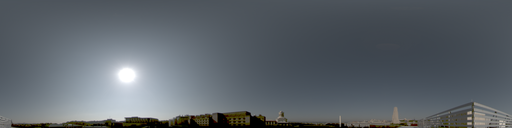
\includegraphics[width=0.16\linewidth]{figures/results/examples/20130621/091938.png} &
%\includegraphics[width=0.2\linewidth]{figures/results/examples/20130621/094937.png} &
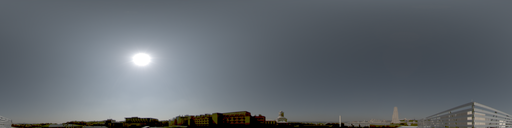
\includegraphics[width=0.16\linewidth]{figures/results/examples/20130621/101936.png} &
%\includegraphics[width=0.2\linewidth]{figures/results/examples/20130621/104435.png} &
%\includegraphics[width=0.2\linewidth]{figures/results/examples/20130621/111434.png} &
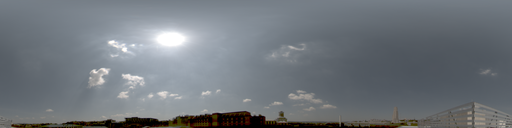
\includegraphics[width=0.16\linewidth]{figures/results/examples/20130621/113934.png} &
%\includegraphics[width=0.2\linewidth]{figures/results/examples/20130621/120933.png} &
%\includegraphics[width=0.2\linewidth]{figures/results/examples/20130621/123933.png} &
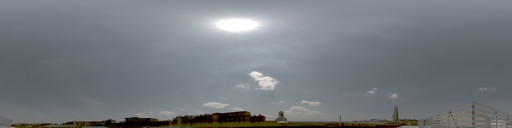
\includegraphics[width=0.16\linewidth]{figures/results/examples/20130621/130433.png} &
%\includegraphics[width=0.2\linewidth]{figures/results/examples/20130621/133432.png} &
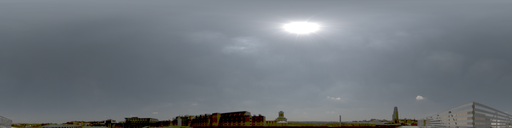
\includegraphics[width=0.16\linewidth]{figures/results/examples/20130621/140431.png} &
%\includegraphics[width=0.2\linewidth]{figures/results/examples/20130621/144650.png} &
%\includegraphics[width=0.2\linewidth]{figures/results/examples/20130621/145704.png} &
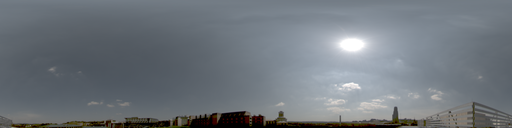
\includegraphics[width=0.16\linewidth]{figures/results/examples/20130621/152700.png} \\%\includegraphics[width=0.2\linewidth]{figures/results/examples/20130621/155157.png} &
%\includegraphics[width=0.2\linewidth]{figures/results/examples/20130621/161154.png} \\

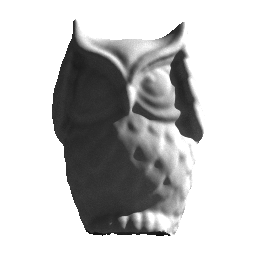
\includegraphics[width=0.16\linewidth]{figures/results/examples/20130621_inputs_owlie/img-01.png} &
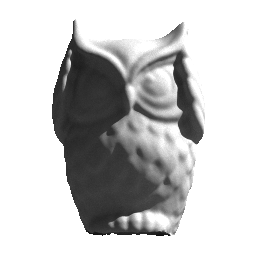
\includegraphics[width=0.16\linewidth]{figures/results/examples/20130621_inputs_owlie/img-03.png} &
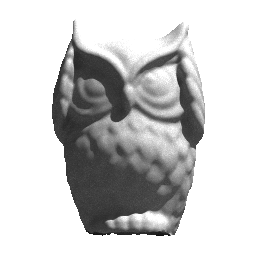
\includegraphics[width=0.16\linewidth]{figures/results/examples/20130621_inputs_owlie/img-06.png} &
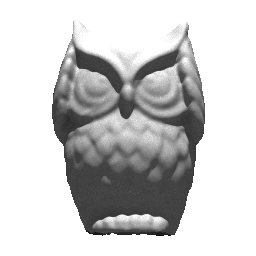
\includegraphics[width=0.16\linewidth]{figures/results/examples/20130621_inputs_owlie/img-09.png} &
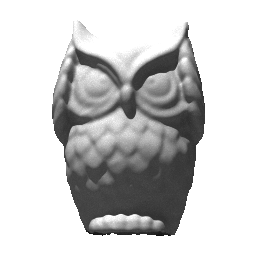
\includegraphics[width=0.16\linewidth]{figures/results/examples/20130621_inputs_owlie/img-11.png} &
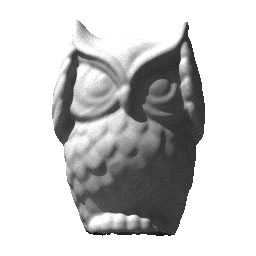
\includegraphics[width=0.16\linewidth]{figures/results/examples/20130621_inputs_owlie/img-14.png} \\
\end{tabular*}

\noindent\rule{0.95\linewidth}{0.4pt}
\newcommand{\reswidth}{0.141}
\begin{tabular*}{\linewidth}{@{}c@{}c@{}c@{}c@{}c@{}c@{}c@{}}
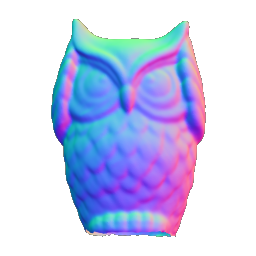
\includegraphics[width=\reswidth\linewidth]{figures/results/examples/gt_owlie_normals.png} &
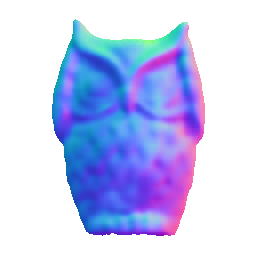
\includegraphics[width=\reswidth\linewidth]{figures/results/examples/ours_owlie_normals.png} &
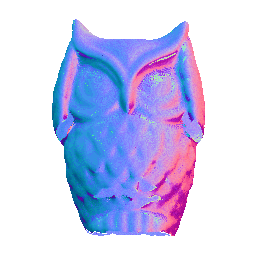
\includegraphics[width=\reswidth\linewidth]{figures/results/examples/jung_owlie_normals.png} &
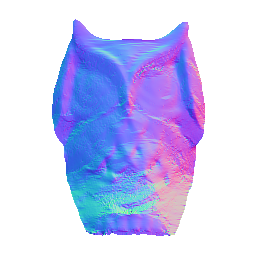
\includegraphics[width=\reswidth\linewidth]{figures/results/examples/yu_owlie_normals.png} &
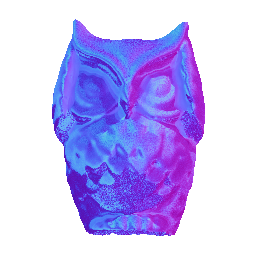
\includegraphics[width=\reswidth\linewidth]{figures/results/examples/dpsn_owlie_normals.png} &
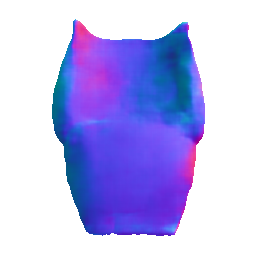
\includegraphics[width=\reswidth\linewidth]{figures/results/examples/marrnet_owlie_normals.png} &
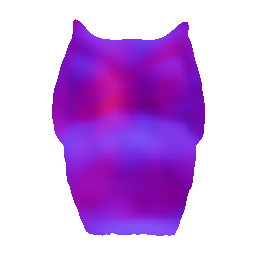
\includegraphics[width=\reswidth\linewidth]{figures/results/examples/ef_owlie_normals.png} \\

\multicolumn{1}{r}{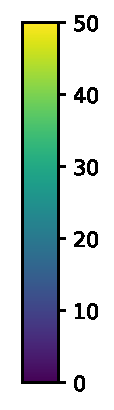
\includegraphics[height=\reswidth\linewidth]{figures/results/examples/colorbar_error_vertical.pdf}} &
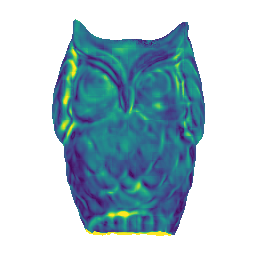
\includegraphics[width=\reswidth\linewidth]{figures/results/examples/ours_owlie_errors.png} &
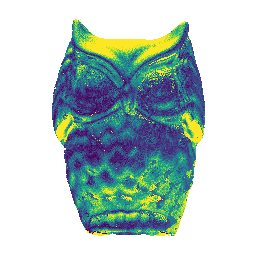
\includegraphics[width=\reswidth\linewidth]{figures/results/examples/jung_owlie_error.png} &
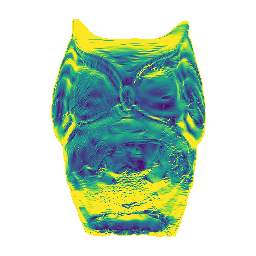
\includegraphics[width=\reswidth\linewidth]{figures/results/examples/yu_owlie_errors.png} &
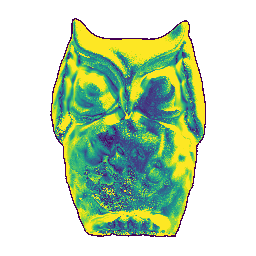
\includegraphics[width=\reswidth\linewidth]{figures/results/examples/dpsn_owlie_errors.png} &
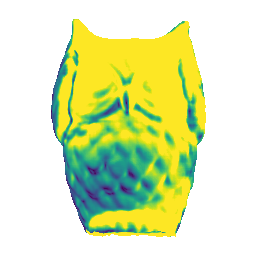
\includegraphics[width=\reswidth\linewidth]{figures/results/examples/marrnet_owlie_errors.png} &
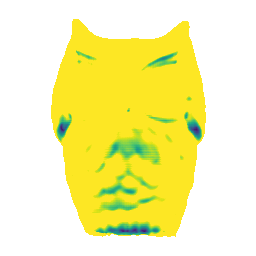
\includegraphics[width=\reswidth\linewidth]{figures/results/examples/ef_owlie_errors.png} \\

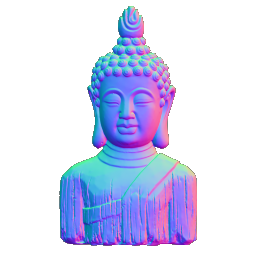
\includegraphics[width=\reswidth\linewidth]{figures/results/examples/gt_buddha_normals.png} &
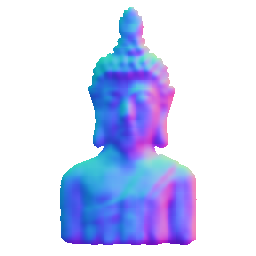
\includegraphics[width=\reswidth\linewidth]{figures/results/examples/ours_buddha_normals.png} &
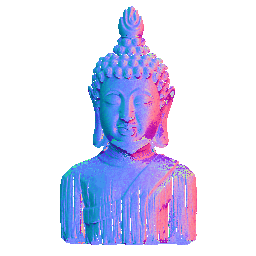
\includegraphics[width=\reswidth\linewidth]{figures/results/examples/jung_buddha_normals.png} &
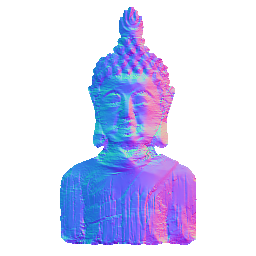
\includegraphics[width=\reswidth\linewidth]{figures/results/examples/yu_buddha_normals.png} &
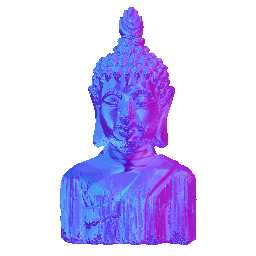
\includegraphics[width=\reswidth\linewidth]{figures/results/examples/dpsn_buddha_normals.png} &
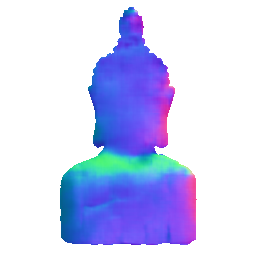
\includegraphics[width=\reswidth\linewidth]{figures/results/examples/marrnet_buddha_normals.png} &

\includegraphics[width=\reswidth\linewidth]{figures/results/examples/ef_buddha_normals.png} \\

\multicolumn{1}{r}{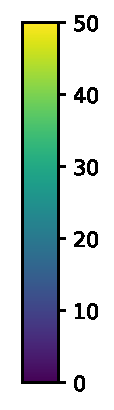
\includegraphics[height=\reswidth\linewidth]{figures/results/examples/colorbar_error_vertical.pdf}} &
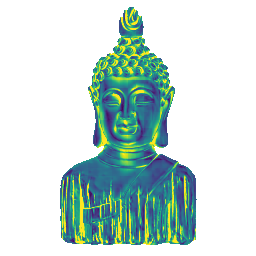
\includegraphics[width=\reswidth\linewidth]{figures/results/examples/ours_buddha_errors.png} &
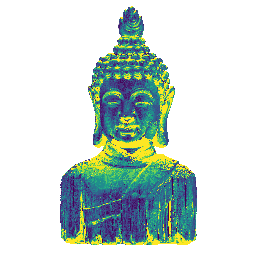
\includegraphics[width=\reswidth\linewidth]{figures/results/examples/jung_buddha_error.png} &
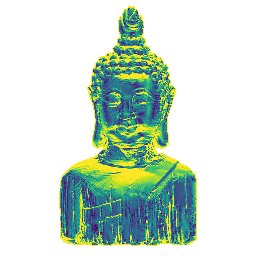
\includegraphics[width=\reswidth\linewidth]{figures/results/examples/yu_buddha_errors.png} &
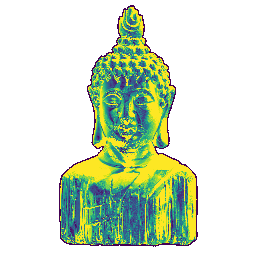
\includegraphics[width=\reswidth\linewidth]{figures/results/examples/dpsn_buddha_errors.png} &
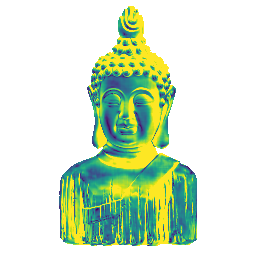
\includegraphics[width=\reswidth\linewidth]{figures/results/examples/marrnet_buddha_errors.png} &
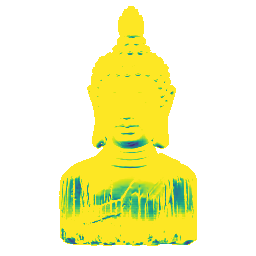
\includegraphics[width=\reswidth\linewidth]{figures/results/examples/ef_buddha_errors.png} \\
\begin{tabular}{@{}c@{}}ground\\truth\end{tabular} & ours & \cite{jung-cvpr-15} & \cite{yu-iccp-13} & \cite{santo-iccv-17} & \cite{wu-nips-17} & \cite{eigen-iccv-15} \\
\end{tabular*}
\egroup
\caption[Lighting environment maps and renders throughout a day]{(top) An example of the lighting environment maps and renders throughout a day. (bottom) Qualitative results (odd rows) and errors in degrees (even rows) of our technique and the state-of-the-art on single-day photometric stereo in the semi-calibrated~\cite{jung-cvpr-15} and calibrated~\cite{yu-iccp-13} cases, deep photometric stereo~\cite{santo-iccv-17} and single image normal estimation~\cite{wu-nips-17,eigen-iccv-15} (averaged over the day) on our real lighting dataset. \textbf{More results available in the supplementary material.}}
\label{fig:results-qualitative}
\end{figure}


In this section, we assess the performance of our method and compare it extensively to the state-of-the-art methods in single-day and regular photometric stereo, as well as some recent single image normal estimation techniques.

\subsection{Evaluation dataset}
\label{sec:evaluation_dataset}

To evaluate and compare the techniques, we rely on a dataset of synthetic objects, lit by real skies. To generate the images, we manually selected 3 sunny days over 2 geographical locations from the Laval HDR sky database~\cite{hdrdb}, which contains unsaturated HDR, omnidirectional photographs of the sky captured with the approach proposed in \cite{stumpfel-afrigraph-04}. We build a virtual 3D scene containing the HDR sky environment map as the sole light source, a 3D object viewed by an orthographic camera, and a 0.3 albedo ground plane placed under the object, outside the field of view of the camera. We used the 3D models from the validation set which the neural network never saw during training. This results in a dataset of 960 renders yielding 60 normal maps to evaluate. Example images obtained with this technique are shown in fig.~\ref{fig:results-qualitative}. 

% High dynamic range (HDR) captures of the sky hemisphere that span the full 22 stops required to properly capture outdoor lighting were taken using the approach proposed in~\cite{stumpfel-afrigraph-04}. We captured three different sunny days over two different geographical locations. 

%Days used: 2013-06-21 (Pittsburgh), 2015-05-14 and 2016-06-17 (Québec City). The sun has a maximum elevation of $73.00\degr$, $61.86\degr$ and $66.59\degr$, respectively.


\subsection{Results and comparisons}

We compare our method to several state-of-the-art techniques relying on photometric stereo and/or deep learning to estimate surface normals from images. For PS techniques, we compare to the calibrated technique of Yu et al.~\cite{yu-iccp-13}, which requires knowledge of the full environment map used to light the object. In our work, we use the variant proposed by Hold-Geoffroy et al.~\cite{holdgeoffroy-3dv-15} and without the low-rank matrix completion preprocessing, which was shown to yield slightly improved results over the original formulation. We also compare to the semi-calibrated method of Jung et al.~\cite{jung-cvpr-15}, which requires only knowledge of the capture geolocation. For deep learning techniques, we compare to the recent Deep Photometric Stereo Network (DPSN)~\cite{santo-iccv-17}, which operates on one pixel at a time. Since it assumes known point light source lighting, we re-trained this model using the sun position from a geographical location and date representative of our training dataset. In addition, we also compare to single image networks: Eigen and Fergus~\cite{eigen-iccv-15} and MarrNet~\cite{wu-nips-17}. Since they rely on a single image, we take the mean of their results averaged over all 8 inputs. 

The comparative results, shown qualitatively in fig.~\ref{fig:results-qualitative} and quantitatively in fig.~\ref{fig:results-quantitative}, clearly demonstrate that our approach significantly outperforms all other techniques. We observe that both single image techniques do not work well and result in very high median errors of around $40\degr$ and $70\degr$ for~\cite{wu-nips-17} and \cite{eigen-iccv-15}, respectively. For \cite{eigen-iccv-15}, this is probably due to the fact that they cannot handle the harsh shadows created by outdoor lighting during sunny days, since they train with indoor lighting only. In addition, MarrNet~\cite{wu-nips-17} outputs a voxel occupation grid and only produces normals as a byproduct (in its latent stage). As such, this method may not be fully optimized for normal estimation.

The PS techniques yield much better results but still yield quite significant error since sunny days do not contain sufficient constraints to accurately recover surface normals. The calibrated method of Yu et al.~\cite{yu-iccp-13} is comparable to the results obtained by DPSN, with a median normal angular estimation error of $33\degr$. Interestingly, the semi-calibrated method of Jung et al.~\cite{jung-cvpr-15} actually yields better results with a median error of $22\degr$, despite needing less information than the calibrated methods. This could be due to its reliance on a parametric clear sky model to estimate lighting, which closely matches the actual ground truth lighting, and to its reliance on an intensity profile matching algorithm.


\begin{figure}[t]
\centering
\includegraphics[width=0.75\linewidth]{figures/results/real_lighting_performance.pdf}
\caption[Reconstruction error on real lighting]{Median reconstruction error on our real lighting dataset displayed vertically as “box-percentile plots”~\cite{esty-jss-03}; the center horizontal bars indicate the median, while the bottom (top) bars are the 25th (75th) percentiles. Our proposed method (green) provides state-of-the-art performance compared to non-learned methods for single-day PS (blue~\cite{jung-cvpr-15}, orange~\cite{yu-iccp-13}), deep learning methods on calibrated photometric stereo (red~\cite{santo-iccv-17}) and single image normals reconstruction (purple~\cite{wu-nips-17}, brown~\cite{eigen-iccv-15}).}
\label{fig:results-quantitative}
\end{figure}

It is interesting to note that most PS techniques capture with some degree of success the left/right component of the surface normals (roughly speaking, the red and blue tints in the normal maps). This axis happens to be the same as the sun trajectory through the day when the camera is facing north or south. This results in strong photometric constraints on this axis. On the other hand, the recovery of the up/down axis is much less successful on most techniques as outdoor photometric cues lack information in this direction through a single sunny day.

In contrast, our method yields a normal map that is, although a bit smoother, qualitatively very similar to the ground truth. Quantitatively, our approach achieves a median error of $14\degr$ over the evaluation set, with the majority of errors being completely below that of the next-best performing method, Jung et al.~\cite{jung-cvpr-15} (see fig.~\ref{fig:results-quantitative}). Even if it is trained on purely synthetic data, our network is able to generalize well to images rendered with real lighting. The difference in performance with respect to DPSN shows the usefulness of dealing with image patches, which allows the network to learn appropriate patch-based shape priors which can be exploited when the photometric cue alone is not sufficient. 

% deep learning based photometric stereo~\cite{santo-iccv-17} as well as two recent single image normals estimation techniques: Eigen and Fergus~\cite{eigen-iccv-15} and MarrNet~\cite{wu-nips-17}. Qualitative results as well as quantitative results on median estimation error are shown in fig.~\ref{fig:experimental_results}-~\ref{fig:performance_real_lighting}, respectively. We observe that our proposed method outperforms previous work the vast majority of the time.


% Deep Photometric Stereo Network (DPSN)~\cite{santo-iccv-17} needs fully calibrated lighting positions. To evaluate on the one-day case, we trained this model using the sun position from a random geographical location and date. The model overfitted to this specific lighting pattern and did not adapt to different geographical locations and dates.

% In the case of~\cite{jung-cvpr-15}, the performance is reported on a subset of 2 objects over 2 days, and the MRF refinement post-processing was not performed. % Calibrated one-day photometric stereo~\cite{yu-iccp-13} was performed without the low-rank matrix completion preprocessing.

% ~\cite{yu-iccp-13,santo-iccv-17,jung-cvpr-15} all infer normals by looking at the photometric cues from a single pixel at a time. We argue that spatiality is important for one-day photometric stereo as it improves the signal-to-noise ratio in the axis perpendicular to the sun path through the day.



%\begin{figure}
%\centering
%\includegraphics[width=0.49\linewidth]{figures/analysis/perfs_per_direction_normal.pdf}
%\includegraphics[width=0.49\linewidth]{figures/analysis/perfs_per_direction_16divs.pdf}
%\hspace*{0.7cm}\begin{tabular*}{0.55\linewidth}{c@{\extracolsep{\fill}}c}
%(a) & (b)
%\end{tabular*} \\
%\caption{Reconstruction performance on our synthetic test dataset in function of the ground truth surface normal direction for our model with regular image input (a) and denominator images input (b).
%\todo{Should we keep this figure?}}
%\label{fig:surface_normal_direction}
%\end{figure}

